\documentclass[a4paper,12pt]{article} % must appear at the beginning of every latex file
\usepackage{color}
\usepackage{graphicx}
\usepackage{float}
\usepackage{minted}
\usepackage{hyperref}
\setminted{breaklines=true, tabsize=2, breaksymbolleft=}
\begin{document}
\title{Database Design And Implementation For E-Commerce}
\author{\small{Sourabh Aggarwal (111601025), Nikhil Kumar Yadav (111601013)}}
\date{\today}
\maketitle
\pagenumbering{roman}
\tableofcontents
\newpage
\pagenumbering{arabic}
\section{Contribution}
As of now, we did everything together.
\section{Introduction}

\subsection{Requirements}
Following is the list of requirements.

\begin{enumerate}
\item Company maintains the details of stock like their id, name, quantity, rating etc.

\item Company maintains the details of users like their id, name, address, phone number, ewallet.

\item Only users which have purchased the product can leave rating and review to product, they can also give rating to the seller. Thus users should also be able to see their past puchases.

\item Users can add balance to their ewallet.

\item Company maintains the details of its suppliers like their id, name, address, phone number and rating. Each supplier has at least some stock for some item. (Suppliers can add new product (stock) and mention its quantity which he/she has.)

\item When users browses for a product, suppliers will be listed based on the quantity user wants.
\end{enumerate}
\section{Entity Relation Diagram}
\begin{figure}[H]
    \centering
    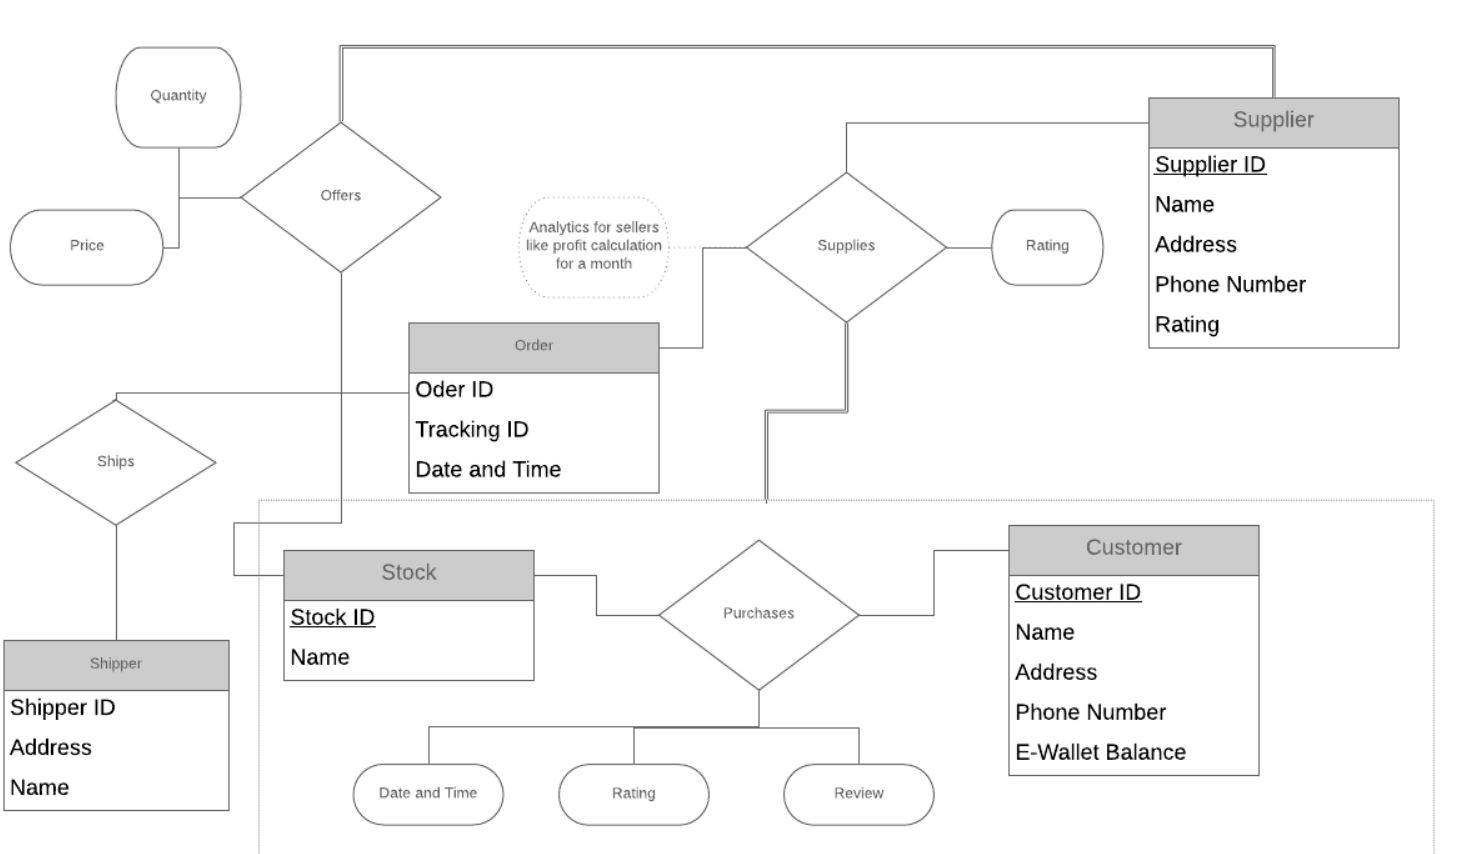
\includegraphics[width=1\textwidth]{ERD2} 
    \caption{Entity Relationship Diagram for e-commerce}
\end{figure}
\section{Database Schema}
\begin{minted}{SQL}

  create table Users (
    username VARCHAR (20) primary key not null,
    passcode VARCHAR (20) not null,
    role VARCHAR (20) not null
  );
  
  create table customer (
    customer_id VARCHAR (20) primary key not null,
    name VARCHAR (20) not null,
    address VARCHAR (60) not null,
    phone_number DECIMAL (10) UNSIGNED not null,
    email_id VARCHAR (20) not null,
    foreign key (customer_id) references Users(username) on delete cascade
  );
  
  create table payment (
    payment_id VARCHAR (20) primary key not null,
    credit_card_number VARCHAR (20) not null,
    date_ timestamp,
    billing_address varchar(60) not null
  );
  
  create table order_ (
    order_id VARCHAR (20) primary key not null,
    customer_id VARCHAR (20),
    shipping_address varchar(60) not null,
    payment_id VARCHAR (20),
    foreign key (customer_id) references customer (customer_id) on delete set null,
    foreign key (payment_id) references payment (payment_id) on delete set null
  );
  
  create table supplier (
    supplier_id varchar (20) primary key not null,
    name varchar (20) not null,
    address varchar (60) not null,
    phone_number decimal (10) UNSIGNED NOT NULL,
    email_id VARCHAR (20) not null,
    foreign key (supplier_id) references Users(username) on delete cascade
  );
  
  create table shipper (
    shipper_id varchar (20) primary key not null,
    name varchar (20) not null,
    head_quarters varchar (60) not null,
    phone_number decimal (10) UNSIGNED not null,
    email_id VARCHAR (20) not null,
    foreign key (shipper_id) references Users(username) on delete cascade
  );
  
  create table track (
    index_ INT AUTO_INCREMENT primary key not null,
    shipper_id varchar (20),
    tracking_id varchar (20),
    foreign key (shipper_id) references shipper (shipper_id) on delete set null
  );
  
  create table product (
    product_id varchar (20) not null,
    supplier_id varchar (20) not null,
    price float not NULL,
    total_stock int,
    description varchar (60),
    foreign key (supplier_id) references supplier (supplier_id) on delete cascade,
    primary key (product_id, supplier_id)
  );
  
  create table product_order (
    product_id varchar(20) not null,
    order_id varchar (20) not null,
    supplier_id varchar (20),
    product_rating int check (product_rating in (1, 2, 3, 4, 5)),
    supplier_rating int check (supplier_rating in (1, 2, 3, 4, 5)),
    ship_index int,
    product_review varchar (60),
    supplier_review varchar (60),
    quantity int,
    primary key (product_id, order_id),
    foreign key (product_id) references product (product_id) on delete cascade,
    foreign key (order_id) references order_ (order_id) on delete cascade,
    foreign key (supplier_id) references supplier (supplier_id) on delete set null,
    foreign key (ship_index) references track (index_) on delete set null
  );
  
\end{minted}
\section{Roles, Triggers, Views}
\subsection{Views}

\begin{itemize}
    \item A view to allow a customer to check his personal previous orders/order history.
    \item A view to check the current status of a particular package.
    \item A view to check the spendings done by the customer per month.
    \item A view for supplier to check his pending (not shipped) packages.
    \item A view for supplier to check his previously processed packages.
    \item A view for supplier to check various important statistics like sale per month. 
    \item A view for shipper to check his not yet delivered packages.
    \item A view for shipper to know his past delivered packages.
    \item A view for shipper to know various statistics like sales per month, sales associated with particular supplier, etc.
\end{itemize}


\subsection{Roles}
\begin{itemize}
    \item A role for database administrator.
    \item A role for customer.
    \item A role for supplier.
    \item A role for shipper.
\end{itemize}

\subsection{Triggers}

\begin{itemize}
    \item Trigger to notify addition of a new customer.
    \item Trigger to notify addition of a new supplier.
    \item Trigger to notify addition of a new shipper.
    \item Trigger to notify addition of new item.
    \item A trigger to add a tuple in track relation before an insertion into \textit{product\_order} relation.
    \item Trigger to notify cutomer of successful order.
    \item Trigger to notify supplier about successful dispatch.
    \item Trigger to notify when the stock goes below a specific amount.
    \item Trigger to delete corresponding entries in various tables if the stock decreases to 0.
    \item Trigger to notify customer that the package has been delivered.
    \item Trigger to notify supplier that the package has been recieved.
    \item Trigger to notify supplier that a customer has left a review.
\end{itemize}

\newpage
\section{Use Cases}
Lets for this case assume that we a supplier. We first want to register and then add products to sell.
\begin{figure}[H]
    \centering
    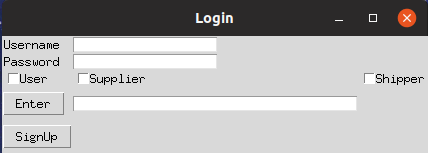
\includegraphics[scale=0.5]{login1.png} 
    \caption{Login page.}
\end{figure}
So at the login page we will select SignUp. It will then open up the SignUp page.
\begin{figure}[H]
    \centering
    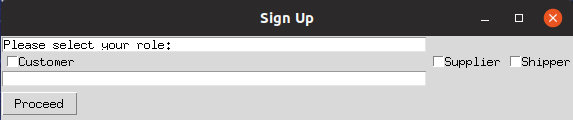
\includegraphics[scale=0.5]{signup1.png}
    \caption{SignUp page(Selecting role).}
\end{figure}
Since we are Supplier we will select supplier option and then proceed.
\begin{figure}[H]
    \centering
    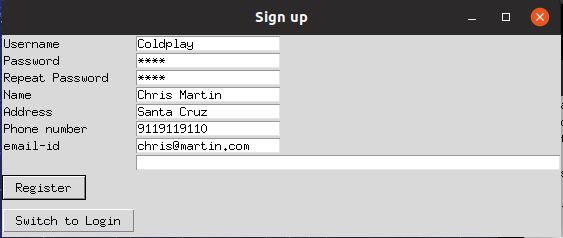
\includegraphics[scale=0.5]{signup2.png}
    \caption{SignUp page(Entering Details).}
\end{figure}
After entering the details press the Register button. It will display that the user is successfully created.
\begin{figure}[H]
    \centering
    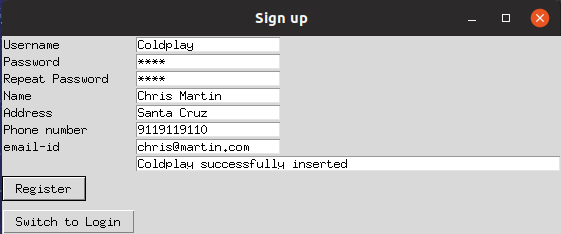
\includegraphics[scale=0.5]{signup3.png}
    \caption{SignUp page(Conformation).}
\end{figure}
After registering goto the login page by pressing the Switch to Login button.
\begin{figure}[H]
    \centering
    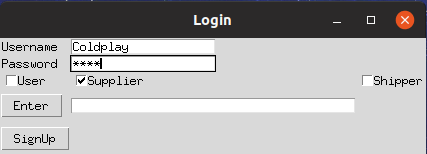
\includegraphics[scale=0.5]{login2.png} 
    \caption{Login page(Entering Details).}
\end{figure}
After login you will be taken to a welcome page which will have two options for you 
\begin{itemize}
    \item Either to add new products in the market.
    \item Or to change the quantites or price of existing products. 
\end{itemize}
\begin{figure}[H]
    \centering
    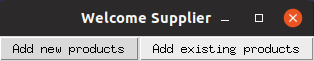
\includegraphics[scale=0.5]{supp1.png} 
    \caption{Welcome page for Supplier.}
\end{figure}
So lets add a new product. You will be taken to a page which will ask to fill the details of the product.
\begin{figure}[H]
    \centering
    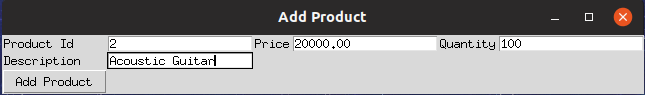
\includegraphics[scale=0.5]{supp2.png} 
    \caption{Add new product.}
\end{figure}
Now the product has been added successfully.

\newpage
\section{Useful links}
\begin{center}
\textbf{Hosted on github with love - } \href{https://github.com/nikhilyadv/DBMS-Lab-Project}{Link}\\
\textbf{GUI source code - } \href{https://github.com/nikhilyadv/DBMS-Lab-Project/GUI}{Link}
\end{center}
\newpage
\section{Logs}
\begin{center}
    **For Developers Use only**
\end{center}
\begin{itemize}
    \item \textbf{$11^{th}Feb2019$ - } \begin{enumerate}
                                          \item Table Schema Modified.
                                          \item Basic Application Interface Completed.
                                          \item Added Use Cases in Report.
                                          \item And yes we are calling it AmaKart.
                                       \end{enumerate}
\end{itemize}

\end{document}